\documentclass[11pt,a4paper]{article}

\usepackage[utf8]{inputenc}
\usepackage[T1]{fontenc}
\usepackage{amsmath,amssymb,amsfonts}
\usepackage{booktabs}
\usepackage{graphicx}
\usepackage{hyperref}
\usepackage[margin=1in]{geometry}
\usepackage{natbib}
\usepackage{array}
\usepackage{tikz}
\usepackage{pgfplots}
\pgfplotsset{compat=1.18}
\usetikzlibrary{patterns,positioning,arrows.meta}

\title{Adaptive Coefficient-Guided Model Trees:\\
Improving the Recursive Hybrid Model with Robust Split Selection}

\author{[Author(s) --- Affiliation(s)]}
\date{}

\begin{document}
\maketitle

\begin{abstract}
Our earlier manuscript introduced the Recursive Hybrid Model (RHM), a minimal linear model tree that selects a splitting feature at each node by fitting Ridge regression and choosing the coefficient with largest absolute magnitude. That baseline is simple and interpretable, but its top-1 coefficient heuristic is brittle under scaling, collinearity, and regime-dependent structure. In this paper we introduce the Adaptive Coefficient-Guided Model Tree (ACGMT), a direct improvement over RHM whose central enhancement is \emph{top-$k$ feature preselection}: instead of committing to a single coefficient-ranked feature, ACGMT screens the top-$k$ candidates and searches each for the best split. We additionally explore node-wise standardization, adaptive coarse-to-fine threshold search, and validation-aware pruning, though ablations show these provide smaller, context-dependent gains. The contribution is not a new model class, but a more robust search strategy for efficient piecewise linear trees. We evaluate ACGMT on five synthetic stress tests (scaling, correlated predictors, irrelevant features, interaction structure, piecewise regimes); because the study is synthetic-only, it isolates specific failure modes but does not constitute a general benchmark. Relative to RHM, top-$k$ screening is the dominant improvement: test MSE drops from 4.746 to 0.385 on the interaction dataset and from 2.791 to 0.352 on the regime dataset. Pruning further improves correlated and regime data (to 0.253 and 0.325), while standardization is neutral to harmful. Gradient boosting remains strongest on the most non-linear settings, but ACGMT is competitive on locally-linear problems while remaining a single interpretable tree.
\end{abstract}

\section{Introduction}

The first paper in this project introduced the Recursive Hybrid Model (RHM), a piecewise linear regression tree that uses Ridge regression twice: first to choose the splitting feature at each node, and then to fit linear models at the leaves \citep{rhm2026}. RHM was intentionally minimal. Its purpose was to show that a coefficient-guided model tree can be implemented cleanly and can outperform a global linear baseline on synthetic non-linear data.

That simplicity, however, comes with a cost. RHM commits to a single splitting feature at each node---the feature with the largest absolute Ridge coefficient---and searches thresholds only along that axis. This top-1 heuristic is computationally attractive, but it is also fragile. Coefficient magnitudes can be distorted by feature scaling, correlated predictors can spread signal across multiple variables, and a coarse threshold grid can miss useful local split points. In short, RHM establishes a baseline, but not yet a robust search procedure.

This paper asks a narrower and more defensible question: can the coefficient-guided idea from RHM be made substantially more robust while preserving the interpretability and efficiency advantages of a single model tree? We answer this by proposing the Adaptive Coefficient-Guided Model Tree (ACGMT), which keeps the overall RHM structure but replaces the top-1 split commitment with a \emph{top-$k$ feature screening} step: the algorithm ranks features by Ridge coefficient magnitude, retains the $k$ highest-ranked candidates, and searches each for the best split. This single change is the paper's central contribution. We additionally explore three supplementary refinements---node-wise standardization, adaptive coarse-to-fine threshold search, and validation-aware pruning---and evaluate when each helps.

The main contribution is empirical and methodological rather than paradigmatic. We do not claim a new model class. Instead, we show that the primary weakness of coefficient-guided model trees is the early commitment to a single splitting feature, and that expanding the search to even $k\!=\!2$ features eliminates most of the failure cases. The supplementary refinements provide smaller, context-dependent gains: adaptive threshold search helps on regime data, pruning gives small regularization benefits on most datasets, and standardization is neutral to harmful. This hierarchy of importance---top-$k$ first, everything else conditional---is itself a key finding.

We evaluate on five synthetic stress tests. The synthetic-only scope is a deliberate choice: it allows us to isolate specific failure modes (scaling, collinearity, irrelevant features, interactions, regime shifts), but the results should not be read as a general benchmark claim. We do not compare against an external exhaustive model-tree implementation in this paper; the focus is on the progression from RHM to ACGMT and on standard tabular baselines.

The paper is organized as follows. Section~\ref{sec:related} positions ACGMT relative to RHM and the broader model-tree literature. Section~\ref{sec:method} defines the proposed method. Section~\ref{sec:experiments} describes the experimental setup. Section~\ref{sec:results} reports the main comparison and ablation results. Section~\ref{sec:discussion} discusses what the experiments imply about coefficient-guided tree construction, and Section~\ref{sec:conclusion} concludes.

\section{Related Work}\label{sec:related}

Model trees extend regression trees by fitting linear models at the leaves rather than constants. Classical CART \citep{breiman1984} performs exhaustive split search and predicts piecewise constants. M5 and M5' \citep{quinlan1992,wang1997} popularized piecewise linear trees with linear leaves and post-hoc smoothing. More recent work includes scikit-learn-compatible linear-tree implementations \citep{cerlymarco2021}, robust fast linear model trees such as PILOT \citep{raymaekers2024}, and performance-oriented systems such as PINE \citep{li2024}.

Our earlier RHM paper \citep{rhm2026} positioned coefficient-guided splitting as a minimal alternative to exhaustive split-feature search. ACGMT is best understood as a direct continuation of that idea rather than a competing paradigm. Relative to RHM, the present paper shifts the emphasis from ``can a top-1 coefficient heuristic work at all?'' to ``how should coefficient-guided search be stabilized and extended?''

We also compare against standard regression baselines beyond the model-tree family. Random forests \citep{breiman2001rf} and gradient boosting regression trees \citep{friedman2001gbm} provide strong non-linear baselines, though at the cost of larger ensembles and lower local interpretability. Our goal is not to replace such methods across the board, but to identify the regime where a single adaptive piecewise linear tree remains competitive.

\section{Method}\label{sec:method}

\subsection{From RHM to ACGMT}

RHM recursively partitions the feature space and fits a local Ridge model at each leaf \citep{rhm2026}. At an internal node, it:
\begin{enumerate}
    \item fits Ridge on the node data;
    \item chooses the feature with largest $|\beta_j|$;
    \item scans a coarse percentile grid on that feature;
    \item recurses on the best split.
\end{enumerate}

ACGMT preserves this overall structure but changes the split search itself. Instead of treating the single largest coefficient as the final split decision, it uses coefficients as a screening device that narrows the search to a small set of plausible features. Figure~\ref{fig:concept} illustrates the difference.

\begin{figure}[ht]
\centering
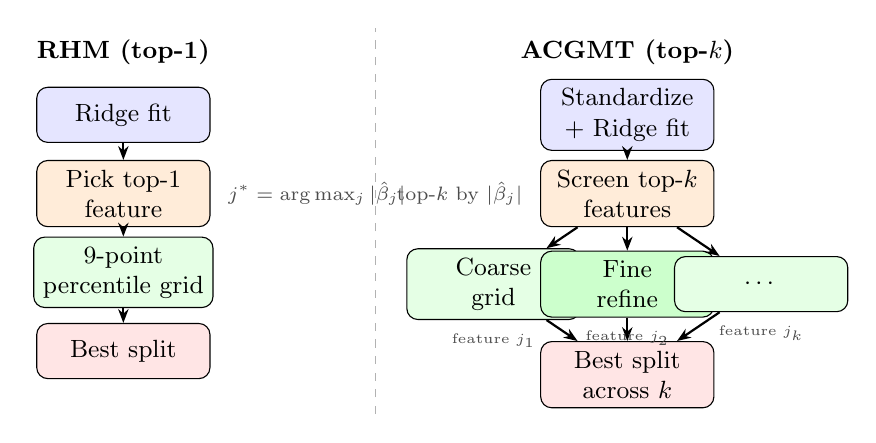
\begin{tikzpicture}[
    box/.style={draw, rounded corners, minimum width=2.2cm, minimum height=0.7cm, font=\small, align=center},
    arrow/.style={-{Stealth[length=5pt]}, thick},
    label/.style={font=\scriptsize, text=black!70},
]
% RHM side
\node[font=\small\bfseries] at (-3.2, 3.8) {RHM (top-1)};
\node[box, fill=blue!10] (r1) at (-3.2, 3) {Ridge fit};
\node[box, fill=orange!15] (r2) at (-3.2, 2) {Pick top-1\\feature};
\node[box, fill=green!10] (r3) at (-3.2, 1) {9-point\\percentile grid};
\node[box, fill=red!10] (r4) at (-3.2, 0) {Best split};

\draw[arrow] (r1) -- (r2);
\draw[arrow] (r2) -- (r3);
\draw[arrow] (r3) -- (r4);
\node[label, right=0.1cm of r2] {$j^* = \arg\max_j |\hat\beta_j|$};

% ACGMT side
\node[font=\small\bfseries] at (3.2, 3.8) {ACGMT (top-$k$)};
\node[box, fill=blue!10] (a1) at (3.2, 3) {Standardize\\+ Ridge fit};
\node[box, fill=orange!15] (a2) at (3.2, 2) {Screen top-$k$\\features};
\node[box, fill=green!10] (a3a) at (1.5, 0.85) {Coarse\\grid};
\node[box, fill=green!20] (a3b) at (3.2, 0.85) {Fine\\refine};
\node[box, fill=green!10] (a3c) at (4.9, 0.85) {$\cdots$};
\node[box, fill=red!10] (a4) at (3.2, -0.3) {Best split\\across $k$};

\draw[arrow] (a1) -- (a2);
\draw[arrow] (a2) -- (a3a);
\draw[arrow] (a2) -- (a3b);
\draw[arrow] (a2) -- (a3c);
\draw[arrow] (a3a) -- (a4);
\draw[arrow] (a3b) -- (a4);
\draw[arrow] (a3c) -- (a4);
\node[label, left=0.1cm of a2] {top-$k$ by $|\hat\beta_j|$};
\node[label, below=0.05cm of a3a, font=\tiny] {feature $j_1$};
\node[label, below=0.05cm of a3b, font=\tiny] {feature $j_2$};
\node[label, below=0.05cm of a3c, font=\tiny] {feature $j_k$};

% Divider
\draw[dashed, black!30] (0, -0.8) -- (0, 4.1);
\end{tikzpicture}
\caption{Conceptual comparison of split selection at a single node. RHM (left) commits to one feature and searches a fixed grid. ACGMT (right) standardizes features, screens the top-$k$ by coefficient magnitude, searches each with optional coarse-to-fine refinement, and selects the best split across all $k$ candidates.}\label{fig:concept}
\end{figure}

\subsection{Algorithm}

Let $(X, y)$ denote the data at a node, with $X \in \mathbb{R}^{n \times d}$ and $y \in \mathbb{R}^n$.

\paragraph{Step 1: coefficient-guided feature screening.}
If standardization is enabled, ACGMT centers and scales the node features column-wise before fitting Ridge. Let $\hat{\beta}$ denote the fitted coefficient vector. The algorithm ranks features by $|\hat{\beta}_j|$ and keeps the top-$k$ candidates rather than only the single largest one.

\paragraph{Step 2: threshold search within screened features.}
For each retained feature, ACGMT first evaluates a coarse quantile grid. In our implementation, the coarse grid matches the 10th through 90th percentiles used by RHM. If adaptive refinement is enabled, the best coarse threshold is then refined by searching a smaller local window with a denser secondary grid.

\paragraph{Step 3: split selection.}
For every candidate threshold $\tau$, the node is partitioned into left and right subsets and two child Ridge models are fit. The score is the weighted in-sample child MSE,
\[
\mathrm{MSE}(\tau) =
\frac{|L| \cdot \mathrm{MSE}_L + |R| \cdot \mathrm{MSE}_R}{n}.
\]
The feature-threshold pair with minimum score is selected, subject to the minimum node size constraint.

\paragraph{Step 4: recursion and pruning.}
Tree growth proceeds recursively until the depth limit or minimum sample constraint is reached. If pruning is enabled, the tree is first grown on a build split and then pruned bottom-up using a held-out validation subset. A subtree is collapsed into a single Ridge leaf whenever the leaf's validation MSE is no worse than the subtree's validation MSE on the validation samples that reach that node.

\subsection{Variants Studied}

The experiments study four ACGMT variants:
\begin{itemize}
    \item \textbf{ACGMT (top1, no-std):} top-$1$ feature selection, no standardization, fixed grid, no pruning. This is the closest ACGMT analogue to RHM.
    \item \textbf{ACGMT (top3, std):} top-$3$ features, standardization, fixed grid, no pruning.
    \item \textbf{ACGMT (full):} top-$3$ features with standardization,
    adaptive threshold refinement, and validation-aware pruning.
    \item \textbf{Ablation variants:} versions that isolate top-$k$, standardization, adaptive grid search, and pruning separately.
\end{itemize}

\subsection{Complexity}

For fixed $k$, fixed coarse grid size, and fixed fine grid size, ACGMT has the same asymptotic training order as RHM up to a larger constant factor. Each internal node now fits one Ridge model for ranking and then evaluates up to $k$ features across a bounded set of candidate thresholds. Thus, compared with RHM, ACGMT spends more computation per node but remains far cheaper than exhaustive search over all features and thresholds. For the settings used here, the practical fit-time overhead is modest relative to gradient boosting, while still preserving the single-tree structure.

\section{Experimental Setup}\label{sec:experiments}

\subsection{Datasets}

We evaluate on five synthetic regression problems designed to stress specific failure modes of coefficient-guided splitting:
\begin{itemize}
    \item \textbf{Scaling:} features live on widely different numeric scales;
    \item \textbf{Correlated:} predictive features are paired with highly correlated surrogates;
    \item \textbf{Irrelevant:} a small number of relevant features are embedded among many irrelevant ones;
    \item \textbf{Interaction:} the response includes regime-dependent interaction effects;
    \item \textbf{Regime:} the response is piecewise linear with multiple breakpoints.
\end{itemize}

Each dataset contains 5{,}000 samples and is split 80/20 into train and test. We run 5 random seeds for every dataset-model pair and report means across seeds.

\subsection{Baselines}

We compare against:
\begin{itemize}
    \item Ridge regression;
    \item CART regression trees;
    \item Random Forest;
    \item Gradient Boosting regression trees;
    \item the original RHM implementation from the first paper \citep{rhm2026}.
\end{itemize}

Random Forest uses single-threaded fitting in order to make fit-time comparisons less misleading. We emphasize fit time rather than prediction time when discussing efficiency, because the current RHM implementation uses slower row-wise prediction while ACGMT uses vectorized prediction.

\subsection{Protocol Details}

All non-pruned ACGMT variants train on the full training set. The pruned \texttt{ACGMT (full)} variant uses an 80/20 build/validation split within the training data, so its tree is grown on 80\% of the nominal training set and pruned using the held-out 20\%. The pruning ablation compares pruned and unpruned models built on the same 80\% subset, so only the pruning step differs.

\section{Results}\label{sec:results}

\subsection{Main Comparison}

Table~\ref{tab:main} reports test MSE and fit time. The headline result is that adaptive coefficient-guided search substantially improves over RHM on datasets where top-1 feature commitment fails, especially the interaction and regime settings. RHM attains test MSE 4.746 on the interaction dataset and 2.791 on the regime dataset, while \texttt{ACGMT (top3, std)} reduces these to 0.385 and 0.352 respectively. The full pruned variant further improves the correlated and regime datasets, reaching 0.253 and 0.325.

\begin{table}[ht]
\centering
\caption{Main comparison across datasets. Test MSE is lower-is-better. Fit time is mean wall-clock training time in seconds.}\label{tab:main}
\resizebox{\textwidth}{!}{
\begin{tabular}{lcccccccc}
\toprule
\textbf{Dataset} & \textbf{Ridge} & \textbf{CART} & \textbf{RF} & \textbf{GBT} & \textbf{RHM} & \textbf{ACGMT top1} & \textbf{ACGMT top3+std} & \textbf{ACGMT full} \\
\midrule
\multicolumn{9}{c}{\textit{Test MSE}}\\
\midrule
correlated  & 0.711 & 2.784 & 2.068 & 0.335 & 0.277 & 0.277 & 0.259 & 0.253 \\
interaction & 5.102 & 1.947 & 1.387 & 0.352 & 4.746 & 4.746 & 0.385 & 0.389 \\
irrelevant  & 1.810 & 7.424 & 5.002 & 0.453 & 0.316 & 0.316 & 0.303 & 0.310 \\
regime      & 2.758 & 0.950 & 0.820 & 0.274 & 2.791 & 2.791 & 0.352 & 0.325 \\
scaling     & 6.492 & 10.649 & 6.833 & 0.615 & 3.020 & 3.020 & 2.963 & 2.998 \\
\midrule
\multicolumn{9}{c}{\textit{Fit time (s)}}\\
\midrule
correlated  & 0.000 & 0.004 & 0.278 & 0.438 & 0.169 & 0.061 & 0.171 & 0.252 \\
interaction & 0.000 & 0.004 & 0.282 & 0.446 & 0.128 & 0.054 & 0.182 & 0.281 \\
irrelevant  & 0.001 & 0.016 & 1.011 & 1.692 & 0.223 & 0.082 & 0.227 & 0.349 \\
regime      & 0.000 & 0.005 & 0.284 & 0.450 & 0.139 & 0.052 & 0.169 & 0.244 \\
scaling     & 0.000 & 0.004 & 0.283 & 0.447 & 0.195 & 0.067 & 0.167 & 0.251 \\
\bottomrule
\end{tabular}}
\end{table}

Figure~\ref{fig:comparison} presents the principal test-MSE comparisons graphically (CART and the top-1 ACGMT variant, which closely tracks RHM, are omitted for clarity). Three comparisons are particularly informative.
First, \texttt{ACGMT (top1, no-std)} closely tracks RHM on every dataset, confirming that the gain does not come merely from reimplementation. Second, \texttt{ACGMT (top3, std)} is the strongest non-pruned variant and delivers the largest improvements over RHM. Third, \texttt{ACGMT (full)} does not uniformly dominate \texttt{top3+std}; pruning and adaptive refinement are useful but context-dependent. This is an important result: the strongest contribution of the paper is not ``adding every enhancement,'' but establishing which enhancements actually matter.

Compared with ensemble baselines, ACGMT occupies a middle ground. Gradient boosting remains best on the most non-linear scaling and interaction problems, but ACGMT is competitive on correlated and irrelevant-feature settings and remains a single interpretable tree rather than an ensemble of many trees.

\begin{figure}[ht]
\centering
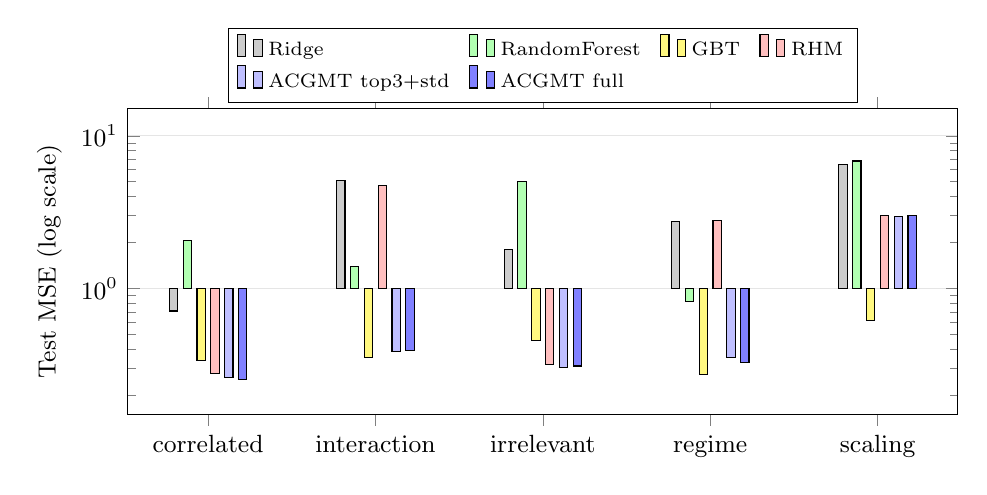
\begin{tikzpicture}
\begin{axis}[
    ybar,
    width=\textwidth,
    height=0.45\textwidth,
    ymode=log,
    ylabel={Test MSE (log scale)},
    symbolic x coords={correlated, interaction, irrelevant, regime, scaling},
    xtick=data,
    x tick label style={font=\small},
    tick label style={font=\small},
    label style={font=\small},
    ymin=0.15, ymax=15,
    bar width=3pt,
    enlarge x limits=0.12,
    legend style={at={(0.5,1.02)}, anchor=south, legend columns=4, font=\scriptsize,
                  /tikz/every even column/.append style={column sep=5pt}},
    legend cell align={left},
    grid=major,
    grid style={gray!20},
    ymajorgrids=true,
    xmajorgrids=false,
]
\addplot[fill=gray!40] coordinates {
    (correlated, 0.711) (interaction, 5.102) (irrelevant, 1.810)
    (regime, 2.758) (scaling, 6.492)};
\addplot[fill=green!30] coordinates {
    (correlated, 2.068) (interaction, 1.387) (irrelevant, 5.002)
    (regime, 0.820) (scaling, 6.833)};
\addplot[fill=yellow!50] coordinates {
    (correlated, 0.335) (interaction, 0.352) (irrelevant, 0.453)
    (regime, 0.274) (scaling, 0.615)};
\addplot[fill=red!25] coordinates {
    (correlated, 0.277) (interaction, 4.746) (irrelevant, 0.316)
    (regime, 2.791) (scaling, 3.020)};
\addplot[fill=blue!25] coordinates {
    (correlated, 0.259) (interaction, 0.385) (irrelevant, 0.303)
    (regime, 0.352) (scaling, 2.963)};
\addplot[fill=blue!50] coordinates {
    (correlated, 0.253) (interaction, 0.389) (irrelevant, 0.310)
    (regime, 0.325) (scaling, 2.998)};
\legend{Ridge, RandomForest, GBT, RHM, ACGMT top3+std, ACGMT full}
\end{axis}
\end{tikzpicture}
\caption{Test MSE comparison across datasets (log scale). RHM fails on the interaction and regime datasets (tall red bars), while ACGMT variants (blue) reduce error by an order of magnitude. GBT (yellow) is strongest on scaling and interaction. ACGMT beats GBT on correlated and irrelevant data.}\label{fig:comparison}
\end{figure}

\subsection{Ablation Study}

Table~\ref{tab:ablations} summarizes the ablations.

\begin{table}[ht]
\centering
\caption{Ablation study: test MSE across datasets.}\label{tab:ablations}
\resizebox{\textwidth}{!}{
\begin{tabular}{lcccccccccc}
\toprule
\textbf{Dataset} & \multicolumn{4}{c}{\textbf{Top-$k$}} & \multicolumn{2}{c}{\textbf{Standardize}} & \multicolumn{2}{c}{\textbf{Grid}} & \multicolumn{2}{c}{\textbf{Pruning}} \\
\cmidrule(lr){2-5}\cmidrule(lr){6-7}\cmidrule(lr){8-9}\cmidrule(lr){10-11}
 & top-1 & top-2 & top-3 & top-5 & no-std & with-std & adaptive & fixed & no-prune & with-prune \\
\midrule
correlated  & 0.265 & 0.259 & 0.259 & 0.259 & 0.259 & 0.259 & 0.259 & 0.259 & 0.263 & 0.253 \\
interaction & 0.528 & 0.385 & 0.385 & 0.385 & 0.385 & 0.385 & 0.374 & 0.385 & 0.388 & 0.389 \\
irrelevant  & 0.336 & 0.310 & 0.303 & 0.304 & 0.303 & 0.303 & 0.304 & 0.303 & 0.316 & 0.310 \\
regime      & 2.441 & 0.352 & 0.352 & 0.353 & 0.352 & 0.352 & 0.337 & 0.352 & 0.331 & 0.325 \\
scaling     & 5.122 & 3.869 & 2.963 & 1.719 & 1.719 & 2.963 & 3.080 & 2.963 & 3.002 & 2.998 \\
\bottomrule
\end{tabular}}
\end{table}

Figures~\ref{fig:topk} and~\ref{fig:ablation_panels} present the ablation results graphically. The ablations support four conclusions.

\paragraph{Top-$k$ screening is the dominant enhancement.}
Moving from top-1 to top-2 or top-3 produces the largest single gains. On the regime dataset, test MSE drops from 2.441 to 0.352; on the interaction dataset it drops from 0.528 to 0.385; on the scaling dataset it drops from 5.122 to 2.963 by top-3 and to 1.719 by top-5. The main weakness of RHM is therefore not merely threshold search, but the early commitment to a single splitting feature.

\paragraph{Standardization is not uniformly helpful.}
We expected node-wise standardization to stabilize coefficient ranking, but in these experiments it is neutral on four datasets and harmful on the scaling stress test. This is a useful negative result. Once top-$k$ screening is already exploring multiple features, naive standardization can alter the ranking in ways that do not improve split quality.

\paragraph{Adaptive threshold search helps when breakpoint precision matters.}
Adaptive refinement improves the regime dataset from 0.352 to 0.337 and the interaction dataset from 0.385 to 0.374, while remaining nearly neutral elsewhere. Its effect is therefore smaller than top-$k$ screening but still meaningful for problems with sharper local transitions.

\paragraph{Pruning is a small but generally positive refinement.}
In the clean pruning ablation, pruning improves correlated, irrelevant, regime, and scaling data, and is effectively neutral on interaction. The gains are modest, which is exactly what one would expect from a bottom-up regularization step rather than a fundamentally different split-selection mechanism.

\begin{figure}[ht]
\centering
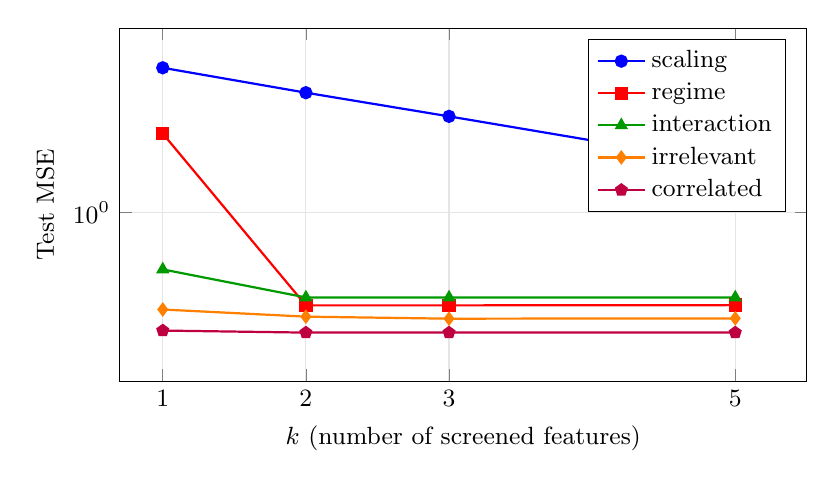
\begin{tikzpicture}
\begin{axis}[
    width=0.85\textwidth,
    height=0.5\textwidth,
    xlabel={$k$ (number of screened features)},
    ylabel={Test MSE},
    ymode=log,
    xmin=0.7, xmax=5.5,
    xtick={1,2,3,5},
    ymin=0.15, ymax=8,
    grid=major,
    grid style={gray!20},
    tick label style={font=\small},
    label style={font=\small},
    legend style={at={(0.97,0.97)}, anchor=north east, font=\small},
    legend cell align={left},
]
\addplot[thick, mark=*, blue] coordinates {(1,5.122) (2,3.869) (3,2.963) (5,1.719)};
\addlegendentry{scaling}
\addplot[thick, mark=square*, red] coordinates {(1,2.441) (2,0.352) (3,0.352) (5,0.353)};
\addlegendentry{regime}
\addplot[thick, mark=triangle*, green!60!black] coordinates {(1,0.528) (2,0.385) (3,0.385) (5,0.385)};
\addlegendentry{interaction}
\addplot[thick, mark=diamond*, orange] coordinates {(1,0.336) (2,0.310) (3,0.303) (5,0.304)};
\addlegendentry{irrelevant}
\addplot[thick, mark=pentagon*, purple] coordinates {(1,0.265) (2,0.259) (3,0.259) (5,0.259)};
\addlegendentry{correlated}
\end{axis}
\end{tikzpicture}
\caption{Effect of top-$k$ feature screening on test MSE (log scale). The largest gains occur from $k\!=\!1$ to $k\!=\!2$. The regime dataset drops from 2.44 to 0.35---a $7\times$ reduction---when the algorithm considers a second feature. Scaling continues to improve through $k\!=\!5$.}\label{fig:topk}
\end{figure}

\begin{figure}[ht]
\centering
\begin{minipage}[t]{0.48\textwidth}
\centering
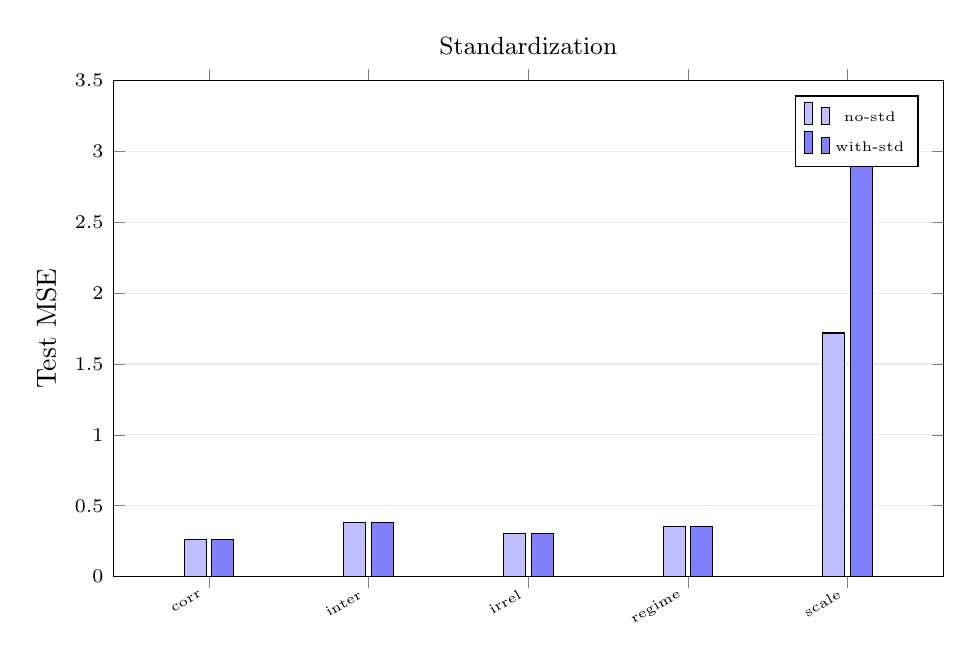
\begin{tikzpicture}
\begin{axis}[
    ybar,
    width=\textwidth, height=0.65\textwidth,
    title={\small Standardization},
    ylabel={Test MSE},
    symbolic x coords={corr, inter, irrel, regime, scale},
    xtick=data,
    x tick label style={font=\tiny, rotate=30, anchor=east},
    tick label style={font=\scriptsize},
    ymin=0, ymax=3.5,
    bar width=8pt,
    enlarge x limits=0.15,
    legend style={at={(0.97,0.97)}, anchor=north east, font=\tiny},
    grid=major, grid style={gray!15}, ymajorgrids=true, xmajorgrids=false,
]
\addplot[fill=blue!25] coordinates {(corr,0.259) (inter,0.385) (irrel,0.303) (regime,0.352) (scale,1.719)};
\addplot[fill=blue!50] coordinates {(corr,0.259) (inter,0.385) (irrel,0.303) (regime,0.352) (scale,2.963)};
\legend{no-std, with-std}
\end{axis}
\end{tikzpicture}
\end{minipage}\hfill
\begin{minipage}[t]{0.48\textwidth}
\centering
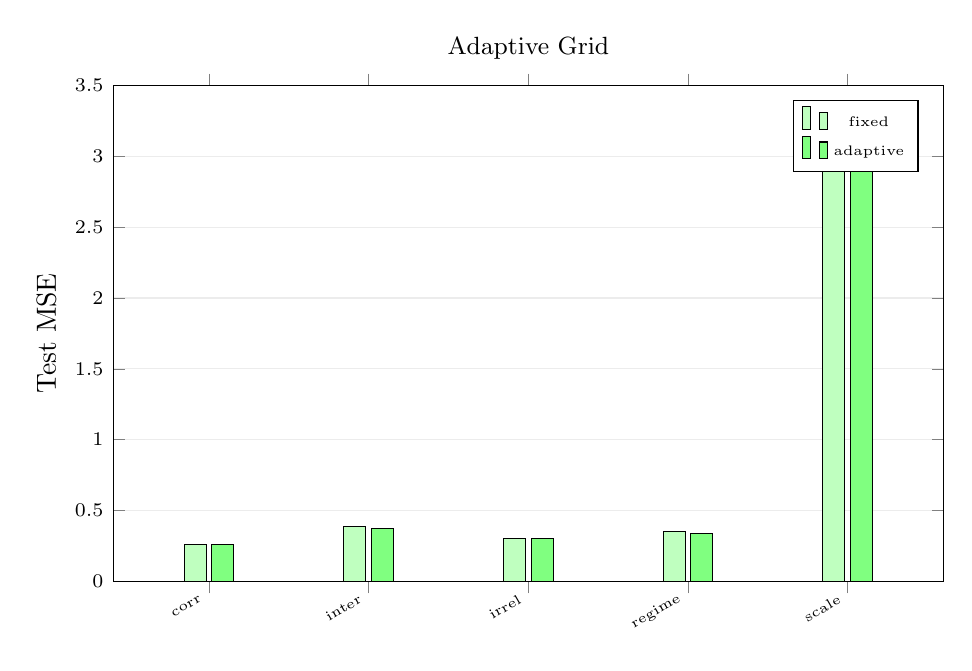
\begin{tikzpicture}
\begin{axis}[
    ybar,
    width=\textwidth, height=0.65\textwidth,
    title={\small Adaptive Grid},
    ylabel={Test MSE},
    symbolic x coords={corr, inter, irrel, regime, scale},
    xtick=data,
    x tick label style={font=\tiny, rotate=30, anchor=east},
    tick label style={font=\scriptsize},
    ymin=0, ymax=3.5,
    bar width=8pt,
    enlarge x limits=0.15,
    legend style={at={(0.97,0.97)}, anchor=north east, font=\tiny},
    grid=major, grid style={gray!15}, ymajorgrids=true, xmajorgrids=false,
]
\addplot[fill=green!25] coordinates {(corr,0.259) (inter,0.385) (irrel,0.303) (regime,0.352) (scale,2.963)};
\addplot[fill=green!50] coordinates {(corr,0.259) (inter,0.374) (irrel,0.304) (regime,0.337) (scale,3.080)};
\legend{fixed, adaptive}
\end{axis}
\end{tikzpicture}
\end{minipage}

\vspace{8pt}

\begin{minipage}[t]{0.48\textwidth}
\centering
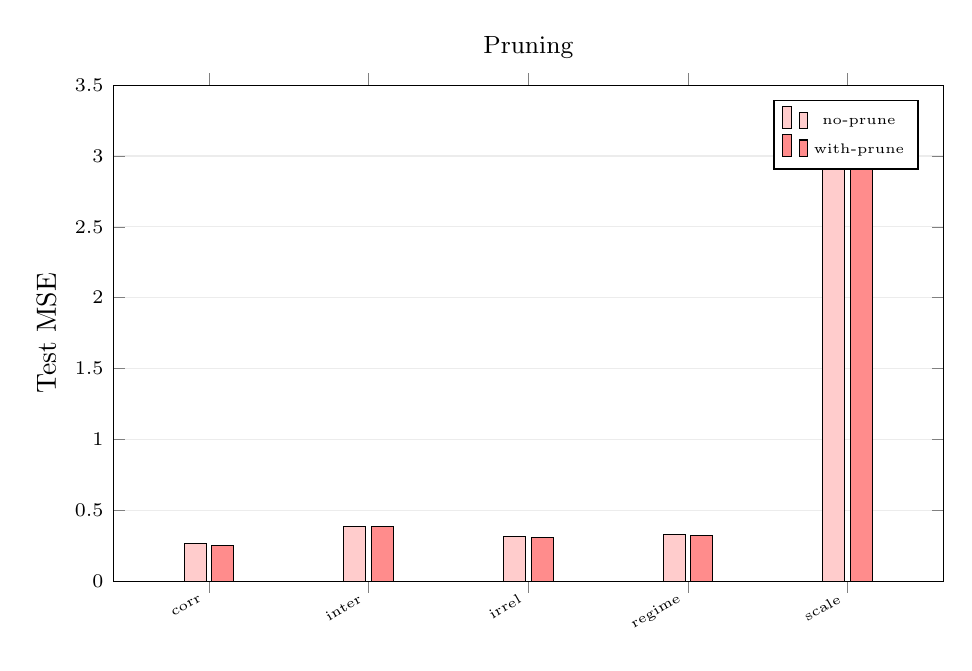
\begin{tikzpicture}
\begin{axis}[
    ybar,
    width=\textwidth, height=0.65\textwidth,
    title={\small Pruning},
    ylabel={Test MSE},
    symbolic x coords={corr, inter, irrel, regime, scale},
    xtick=data,
    x tick label style={font=\tiny, rotate=30, anchor=east},
    tick label style={font=\scriptsize},
    ymin=0, ymax=3.5,
    bar width=8pt,
    enlarge x limits=0.15,
    legend style={at={(0.97,0.97)}, anchor=north east, font=\tiny},
    grid=major, grid style={gray!15}, ymajorgrids=true, xmajorgrids=false,
]
\addplot[fill=red!20] coordinates {(corr,0.263) (inter,0.388) (irrel,0.316) (regime,0.331) (scale,3.002)};
\addplot[fill=red!45] coordinates {(corr,0.253) (inter,0.389) (irrel,0.310) (regime,0.325) (scale,2.998)};
\legend{no-prune, with-prune}
\end{axis}
\end{tikzpicture}
\end{minipage}\hfill
\begin{minipage}[t]{0.48\textwidth}
\centering
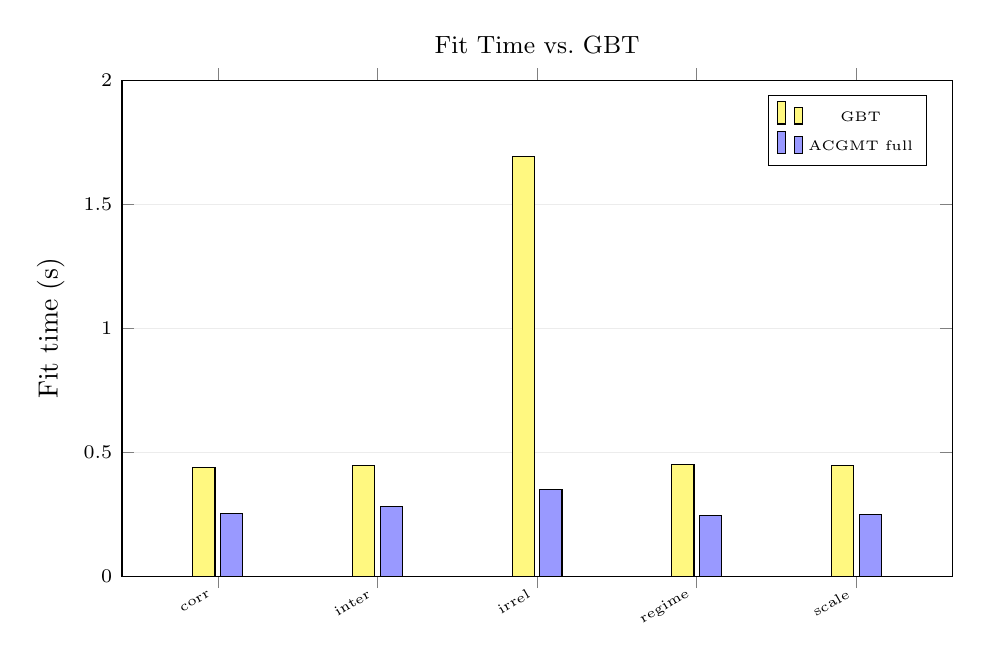
\begin{tikzpicture}
\begin{axis}[
    ybar,
    width=\textwidth, height=0.65\textwidth,
    title={\small Fit Time vs.\ GBT},
    ylabel={Fit time (s)},
    symbolic x coords={corr, inter, irrel, regime, scale},
    xtick=data,
    x tick label style={font=\tiny, rotate=30, anchor=east},
    tick label style={font=\scriptsize},
    ymin=0, ymax=2.0,
    bar width=8pt,
    enlarge x limits=0.15,
    legend style={at={(0.97,0.97)}, anchor=north east, font=\tiny},
    grid=major, grid style={gray!15}, ymajorgrids=true, xmajorgrids=false,
]
\addplot[fill=yellow!50] coordinates {(corr,0.438) (inter,0.446) (irrel,1.692) (regime,0.450) (scale,0.447)};
\addplot[fill=blue!40] coordinates {(corr,0.252) (inter,0.281) (irrel,0.349) (regime,0.244) (scale,0.251)};
\legend{GBT, ACGMT full}
\end{axis}
\end{tikzpicture}
\end{minipage}
\caption{Ablation panels. Top-left: standardization is neutral on 4/5 datasets and harmful on scaling. Top-right: adaptive grid refinement helps regime (0.352$\to$0.337) and interaction (0.385$\to$0.374). Bottom-left: pruning gives small improvements on 4/5 datasets. Bottom-right: ACGMT full fits faster than GBT on all datasets.}\label{fig:ablation_panels}
\end{figure}

\section{Discussion}\label{sec:discussion}

The experiments suggest that coefficient-guided model trees are viable, but only when the coefficient signal is used as a \emph{screening tool} rather than a hard one-feature decision rule. This is the central lesson of the paper. RHM's top-1 heuristic fails badly on interaction and regime data; once the search is expanded to a small set of plausible features, the method becomes far more robust.

The results also clarify what ACGMT is \emph{not}. It is not a universal replacement for strong tree ensembles. Gradient boosting remains superior on the most strongly non-linear scaling and interaction settings. Nor does every proposed enhancement help equally: top-$k$ screening is the clear driver of improvement, adaptive threshold refinement provides targeted gains, pruning gives small regularization benefits, and standardization is at best mixed in the present synthetic suite.

These observations lead to a more precise methodological claim than in the first paper. The value of coefficient-guided model trees lies not in a single heuristic, but in a family of constrained search strategies that trade exhaustive split search for a guided restricted search. ACGMT represents one such strategy.

There are also clear limitations. First, the study is synthetic-only. This is appropriate for isolating failure modes, but not sufficient for broad benchmarking claims. Second, we do not compare against an external exhaustive model-tree implementation in the present paper; the experiments instead focus on standard tabular baselines and direct comparison with RHM. Third, the present implementation still gives RHM a slower prediction path than ACGMT, so fit time is the cleaner efficiency metric.

\section{Conclusion}\label{sec:conclusion}

This paper presented the Adaptive Coefficient-Guided Model Tree (ACGMT), a direct improvement over the Recursive Hybrid Model introduced in our earlier work. ACGMT's central enhancement is top-$k$ feature screening: instead of committing to a single coefficient-ranked feature, the algorithm evaluates the top-$k$ candidates and selects the best split across them. Adaptive threshold refinement and validation-aware pruning provide supplementary, context-dependent gains; standardization is not uniformly beneficial.

The main empirical conclusion is clear: RHM's primary weakness is the early commitment to a single splitting feature, and expanding the search to even $k\!=\!2$ candidates eliminates most failure cases. On difficult interaction and regime datasets, top-$k$ screening alone reduces error by an order of magnitude. The supplementary refinements---adaptive grid search and pruning---contribute smaller improvements on specific datasets. The resulting method remains a single interpretable tree, is faster to fit than gradient boosting in our experiments, and significantly improves over the original coefficient-guided baseline.

The broader implication is that coefficient-guided model trees should be studied as \emph{adaptive search procedures}, not as one-shot heuristics. That reframing is the main improvement over the first paper, and it provides a more credible basis for future work on efficient piecewise linear trees.

\bibliographystyle{plainnat}

\begin{thebibliography}{11}

\bibitem[Breiman et~al.(1984)]{breiman1984}
Breiman, L., Friedman, J., Olshen, R., \& Stone, C. (1984).
\newblock \emph{Classification and Regression Trees}.
\newblock Wadsworth.

\bibitem[Breiman(2001)]{breiman2001rf}
Breiman, L. (2001).
\newblock Random Forests.
\newblock \emph{Machine Learning}, 45(1), 5--32.

\bibitem[Cerlymarco(2021)]{cerlymarco2021}
Cerlymarco. (2021).
\newblock linear-tree: A python library to build Model Trees with Linear Models at the leaves.
\newblock GitHub. \url{https://github.com/cerlymarco/linear-tree}

\bibitem[Friedman(2001)]{friedman2001gbm}
Friedman, J.~H. (2001).
\newblock Greedy Function Approximation: A Gradient Boosting Machine.
\newblock \emph{The Annals of Statistics}, 29(5), 1189--1232.

\bibitem[Li et~al.(2024)]{li2024}
Li, Z., et~al. (2024).
\newblock PINE: Efficient yet Effective Piecewise Linear Trees.
\newblock \emph{SC24 Supercomputing Conference Proceedings}.
\newblock \url{https://sc24.supercomputing.org/proceedings/poster/poster_files/post258s2-file3.pdf}

\bibitem[Quinlan(1992)]{quinlan1992}
Quinlan, J.~R. (1992).
\newblock Learning with Continuous Classes.
\newblock \emph{Proceedings of the 5th Australian Joint Conference on Artificial Intelligence}, 343--348.

\bibitem[Raymaekers et~al.(2024)]{raymaekers2024}
Raymaekers, J., Rousseeuw, P.~J., Verdonck, T., \& Yao, R. (2024).
\newblock Fast Linear Model Trees by PILOT.
\newblock \emph{Machine Learning}.
\newblock \url{https://doi.org/10.1007/s10994-024-06590-3}

\bibitem[Authors(2026)]{rhm2026}
Author(s). (2026).
\newblock A Recursive Hybrid Model for Piecewise Linear Regression: Algorithm Design, Analysis, and Empirical Evaluation.
\newblock Unpublished manuscript.

\bibitem[Wang \& Witten(1997)]{wang1997}
Wang, Y., \& Witten, I.~H. (1997).
\newblock Induction of Model Trees for Predicting Continuous Classes.
\newblock \emph{Proceedings of the European Conference on Machine Learning}, 128--137.

\end{thebibliography}

\end{document}
